\documentclass[10pt,conference]{ieeeconf}

%\usepackage{algpseudocode}% http://ctan.org/pkg/algorithmicx
\usepackage{xcolor}
\usepackage{subfigure}
\usepackage{amsmath,amssymb,amsbsy}
\usepackage{pdfpages}
\usepackage{epstopdf}
\usepackage{color}
\usepackage{fixmath}
\usepackage{optidef}
\usepackage{cite}
\usepackage{array,tabularx}
\usepackage{booktabs}
\usepackage[hidelinks]{hyperref}
\usepackage{cleveref}

\usepackage{color}

\ifpdf
  \RequirePackage{graphicx}
  \RequirePackage{epstopdf}
  \DeclareGraphicsExtensions{.pdf,.jpeg,.png,.jpg}
\else
  \RequirePackage[dvipdfmx]{graphicx}
  \RequirePackage{bmpsize}
  \DeclareGraphicsExtensions{.eps,.pdf,.jpeg,.png,.jpg}
\fi
\graphicspath{{pics/},{./Images/}}

\RequirePackage{algorithm}
\RequirePackage{algorithmic}
\renewcommand{\algorithmicrequire}{\textbf{Input:}}
\renewcommand{\algorithmicensure}{\textbf{Output:}}
\providecommand{\algorithmautorefname}{Algorithm}

\RequirePackage{subfigure}
\RequirePackage{empheq}
\providecommand{\subfigureautorefname}{\figureautorefname}
\Crefname{table}{Table}{Table}
\Crefname{figure}{Fig.}{Fig.}
\Crefname{algorithm}{Algorithm}{Algorithm}

\providecommand{\rm}[1]{\mathrm{#1}}
\providecommand{\od}{\mathrm{d}}

\DeclareMathOperator*{\argmax}{arg\,max}
\DeclareMathOperator*{\argmin}{arg\,min}

\IEEEoverridecommandlockouts
\begin{document}

\title{Multichannel Deconvolution of Skin Conductance Data: Concurrent Separation of Tonic and Phasic Component}
% should be concise and informative to broad readers and attract attention from potential readers.


\author{Yuchen Jin, Jin Lu, Md. Rafiul Amin, and Rose T. Faghih \thanks{Yuchen Jin, Jin Lu, Md. Rafiul Amin, and Rose T. Faghih are with the Department of Electrical and Computer Engineering at the University of Houston, Houston, TX 77004 USA (e-mail: \tt\small  yjin4@uh.edu, jlu28@uh.edu, mamin@central.uh.edu, rtfaghih@uh.edu).} 
}

\maketitle

\begin{abstract}

Understanding the electrodermal activities (EDA) is an essential step in neuroscience. To retrieve the neural events from EDA, one of the key step is the deconvolution. In this work, we decompose the skin conductance (SC) data as a combination of the phasic component and the tonic component. To eliminate the influence of the noise, we utilize multi-channel data and use a multi-channel state-space model to describe the phasic component. To improve the fitness of the tonic extraction, we propose an adaptive bases method and ensure that the appearance of peaks in the tonic component is relatively later than the appearance of the phasic component. To perform the optimization, we adopt the concurrent coordinate descent algorithm, where the phasic component and the tonic component are solved by the interior point method and FOCUSS+ respectively. To determine the proper value of the regularization ratio, we introduce the generalized cross-validation (GCV) in both methods. The experiments show that our method could achieve a good performance. Compared to the results of the conventional tonic extraction method, the fitness of our results is significantly improved.

\end{abstract}

\section{Introduction} \label{introduction}

Analyzing the electrical activities of neurons is (an important aspect in the neuroscience) of great interest in biomedical signal processing. By placing the electrodes, intramuscular needles or some other wearable devices, the neuron activities could be detected by different kinds of indirect methods including the electroencephalogram, electrodermal activities~\cite{savazzi2019estimation,jain2016compressed,amin2019robust}, electromyography signals~\cite{biagetti2016homomorphic}, calcium imaging, and some other approaches. The study of the neural activities could be utilized in many applications, like predicting people's emotions~\cite{feng2018wavelet}, monitoring the health-related abnormal events~\cite{said2017wearable}, and developing the brain-computer interface~\cite{de2018use}.

In this work, we concentrate on the study of electrodermal activities (EDA). One example of EDA is the skin conductance (SC) data, which is collected by detecting activities of people's sweat glands. The sensors for detecting SC could be placed on either the hand palms, fingers, legs or feet. Previous works~\cite{fowles1981publication,amin2019robust} show that the SC of different body parts is controlled by the universal neural signal from the autonomic nervous system (ANS). Within this hypothesis, the whole collection of SC could be modeled as a group of multichannel signals, where one channel represents the collected SC from a specific body part. For any channel $n$, the signal could be formulated by
\begin{align} \label{fml:scmodel}
  y_{\rm{SC}_\mathit{n}}(t) = p_n(t) + s_n(t) + \nu_n(t),
\end{align}
%
where $s_n(t)$ is the tonic component representing the influence of the thermoregulation and general arousal of the
body, $p_n(t)$ is the phasic component thought as reflected from the activity of ANS, and $v_n(t)$ is the additive noise. Different from the slowly drifting tonic component, the phasic component is fast-varying, which makes it possible to separate the two signals by formulating two different mathematical models. Either the tonic component and the phasic component could be regarded as a linear composition of different basis functions, or a group of kernels convoluted with weighted impulse trains. It is possible to formulate a deconvolution problem with the physiological interpretation of SC, which requires a solution for the ANS activation given the composed signal  $y_{\rm{SC}_n}(t)$  is known.

\subsection{Deconvolution}

The neural stimuli from the ANS is though as spike signals. While after the signal is conducted to the sweat glands, the signals are smoothly filtered due to the (physiological effects) physiological systems. After applying the deconvolution, the estimated neural stimuli could be used for denoising, emotion predictions, or health monitoring. \textit{Caruelle et al.}~\cite{caruelle2019use} summarizes the applications of the EDA analysis in recent years. For more details, \textit{Posada et al.}~\cite{posada2020innovations} provides a review on the previous deconvolution methods with the EDA data. Similar to EDA, the other kinds of signals could be also used for studying the neuron activities by deconvolution. In \Cref{tab:literature}, we inspect on several works on deconvolution with different data. For the simplest case, the spike signal could be retrieved by applying a threshold and performing the local maximum searching~\cite{kaur2016remote,subramanian2019systematic}. In most works, the deconvolution is solved by formulating an optimization problem based on a linear model, including the Bateman function~\cite{savazzi2019estimation,greco2014electrodermal,greco2015cvxeda,amin2019tonic,hernando2017feature,wickramasuriya2019skin}, the AR-1 model~\cite{friedrich2017fast}, and the state-space model~\cite{kazemipour2017fast,amin2019robust}. 

\begin{table*}[htbp]
  \centering
  \normalsize
  \caption{A summary of the previous works about deconvolution.}
  \label{tab:literature}
  \begin{tabular}{m{0.14\textwidth}<{\raggedright}m{0.14\textwidth}<{\raggedright}m{0.65\textwidth}}
    \toprule
    \multicolumn{1}{c}{Study} & \multicolumn{1}{c}{Data} & \multicolumn{1}{c}{Methodology} \\ \midrule
    \textit{Friedrich et. al.}~\cite{friedrich2017fast} & Calcium imaging data & The conversion from the calcium spikes to the observed fluorescenc signals is described as an AR-p model. The authors propose an algorithm, OASIS for solving the constrained optimization problem in the AR-1 case. \\
    \textit{Kazemipour et. al.}~\cite{kazemipour2017fast} & Calcium imaging data & Develop a compressible state-space model for describing the data. The spikes are designed as the innovation sequence of the state. The optimization problem is solved by a nested Expectation-Maximization algorithm. \\
    \textit{Kaur et. al.}~\cite{kaur2016remote} & Electro-cardiogram & Introduce two methods. The first method is based on curve fitting and local maximum searching. The second method is Blind Deconvolution, where the kernel and the spikes are optimized alternatively. \\
    \textit{Mesin}~\cite{mesin2019single} & Electromyogram & Model the EMG signal by motor unit kernels. The deconvolution is performed by solving an $\ell_1$ regularized optimization problem by the iterative reweighted least square algorithm. \\
    \textit{Antink et. al.}~\cite{friedrich2017fast} & ECG, ABP and PPG & The author use the blind deconvolution to solve the heart beat spikes. This paper introduces a multi-observation scheme by assuming a universal spike data. \\
    \textit{Subramanian et. al.}~\cite{subramanian2019systematic} & EDA & Use a low-pass FIR filter to isolate the tonic component, the spike is found by searching local maximum in phasic component. \\ 
    \textit{Savazzi et. al.}~\cite{savazzi2019estimation} & EDA & The tonic component and noise is removed by a low-pass FIR filter. The phasic component is modeled by Bateman function. The spike is acquired by optimization. \\ 
    \textit{Jain et. al.}~\cite{jain2016compressed} & EDA & Involve the compress sensing into the deconvolution. The optimization is performed on the differential signal to eliminate the influence of sudden changes of the tonic component. \\
    \textit{Greco et. al.}~\cite{greco2014electrodermal} & EDA & The tonic component is estimated by Gaussian smoothing and interpolation. The spike is solved by modeling the phasic component with Bateman function. \\ 
    \textit{Greco et. al.}~\cite{greco2015cvxeda}, \textit{Amin and Faghih}~\cite{amin2019tonic} & EDA & Model the phasic component and the tonic component by Bateman function and spline function respectively, then formulate the deconvolution as a joint constrained convex optimization problem. \\ 
    \textit{Hernando et. al.}~\cite{hernando2017feature} & EDA & The tonic and phasic components are decomposed by two groups of pre-defined bases. The phasic component basis is designed by using Bateman function. \\
    \textit{Wickramasuriya et. al.}~\cite{wickramasuriya2019skin} & EDA & The tonic component is isolated by using cvxEDA~\cite{greco2015cvxeda}. The phasic component is decomposed by a basis based on Bateman function. The deconvolution is solved by a hybrid algorithm based on GCV and FOCUSS+. \\
    \textit{Amin and Faghih}~\cite{amin2019robust} & EDA & The authors propose a multichannel deconvotion scheme. The tonic component is removed by using cvxEDA~\cite{greco2015cvxeda} on each channel, and the phasic component is formulated by a state-space model. The deconvolution is solved by the hybrid algorithm GCV-FOCUSS+. \\ \bottomrule
  \end{tabular}
\end{table*}

The complexity of the deconvolution differs in different applications. In \cite{greco2015cvxeda}, the basis determining the shape of the phasic component is fixed, while in \cite{hernando2017feature}, the phasic component is modeled by several fixed bases. In \cite{greco2014electrodermal,amin2019tonic,wickramasuriya2019skin,kazemipour2017fast,amin2019robust}, although there is a single basis, the shape of the basis could be learned. Particularly, some researches assume that the linear model is totally unknown. By only giving an initial guess, the modeling function is also optimized by blind deconvolution~\cite{kaur2016remote,friedrich2017fast}. For a large scale application, the problem requires to be formulated properly according to the computational consumption.

Most of the mentioned works deal with single channel data, while in \cite{friedrich2017fast,amin2019robust}, a multichannel scheme is introduced for improving the robustness of the predictions. In the practice, observations are contaminated with the noise, which may influence the accuracy of the deconvolved spikes. The motivation of introducing multichannel data is based on the hypothesis that the same neural stimuli is shared by the data acquired by different observations. When the multichannel data is deconvolved jointly, the noise from different channels could be attenuated by each other, thus the problem could converge towards a better solution.

\subsection{Tonic separation}
 
Previously there some works on the tonic component separation. In \cite{van1967skin}, the raw EDA signal is decomposed as absolute change in conductance, change as a ratio of the basic conductance level (BLC), and log conductance change. In \cite{green2014development}, the author proposes a method of automated analysis of SCR data in the contexts of event-related cognitive tasks and nonspecific responding to complex stimuli. \cite{greco2014electrodermal} formulates the separation as a quadratic programming problem, where the phasic component and the tonic component are decomposed by the basis of the biexponential Bateman functions and the B-spline functions respectively. To solve the problem that the tonic component may overlap each other, \textit{Vartak et. al.}~\cite{vartak2009estimation} proposes a mathematical model fitting procedure is used to separate these overlapping components. Features are extracted using the mathematical model fitting procedure. In~\cite{amin2019tonic}, the author proposes a generalized-cross-validation-based block coordinate descent approach. In this approach, the tonic component is regarded as a summation of a series of P shifted and weighted cubic B-spline functions. Then the problem is solved by minimizing an $\ell_p$ penalized loss function. Especially, inspired by compress sensing, \textit{Jain et. al.}~\cite{jain2016compressed} builds a model for separating the difference of the signal instead of the raw signal. This idea is effective for eliminating the interference caused by sudden changes of the tonic component.

In some previous works, the tonic component separation and the phasic component deconvolution are performed individually~\cite{greco2014electrodermal,amin2019robust}. Since both the modeling method and the inversion method in \cite{amin2019robust} are designed for the multichannel case, the previous tonic separation works designed for single-channel data may cause deviation for the solution. In addition to the motivation, we are interested in multi-channel deconvolution inorder to obtain more accurate results in presence of noise. As tonic component separation is performed separately, inaccuracy in separation in presence of artifact and noise may lead to inaccurate deconvolution of ANS activation. A multi-channel tonic and phasic decomposition may lead to a more robust decomposition in presence of noise. In our work, we extend the multichannel deconvolution into the joint optimization for solving the tonic component in the multichannel case. With this scheme, the neural stimuli from the ANS is though to be shared, while the solution for the composition of tonic basis is assumed to be different in different channels. To improve the fitness of the tonic component, we propose a new method for generating the B-spline bases based on the solve neural stimuli. The results show that our method could achieve a better performance.

\section{Theory}

According to \eqref{fml:scmodel}, the SC data could be decomposed into a tonic component and a phasic component. In this work, we will model both components by different methods. The phasic component is decomposed by a series of state-space models sharing the same input, while the tonic component is described as a combination of different spline functions. Based on the theory-based multichannel forward modeling, the stimuli from the ANS could be solved by a joint optimization. In the meanwhile, the tonic component would be extracted from the data.

\subsection{Model the phasic component with a multichannel state-space representation}
According to the presumption in \cite{alexander2005separating,society2012publication,amin2019robust}, the phasic components detected in different regions of the body are regulated by the same ANS signal, the detected phasic component for channel $n$ could be formulated by
\begin{align}
p_n(t) = \alpha_n \zeta_n (t),
\end{align}
where $\alpha_n$ denotes the attenuation rate compared to the first channel. This attenuation is caused by the the different number and sizes of sweat glands in different location. In this configuration, $\alpha_1$ is fixed on 1.0. $\zeta_n(t)$ is an internal variable which is modeled by a smoothing filter applied to the neural stimuli $u(t-\beta_n)$. The conduction delay $\beta_n$ shows that the
same stimuli would be detected at different times at different locations. We follow the configurations in \cite{greco2015cvxeda,amin2019robust} and model the neural stimuli by a series of spikes with the sparse constraint, i.e. $u(t) = \sum_{i=1}^N q_i \delta(t - \Delta_i)$, where $q_i$ is the spike signal in time interval i, and $\Delta_i$ is the time for $i^{\mathrm{th}}$ time interval. Given $u(t)$, \textit{Alexander et al.}~\cite{alexander2005separating} provides a second-order ordinary differential equation to describe $\zeta_n(t)$,
\begin{align} \label{fml:the:ode}
\tau_r \tau_d \frac{\od^2 \zeta_n(t)}{\od t^2} + (\tau_r + \tau_d) \frac{\od \zeta_n(t)}{\od t} + \zeta_n(t) = u(t - \beta_n).
\end{align}
where $\tau_r$ and $\tau_d$ represent the rise and decay times respectively.

The difference between different channels in \eqref{fml:the:ode} is only the time delay. In other words, the solutions of $\zeta_n(t)$ for different $n$ are the same except the time delay. According to \eqref{fml:the:ode}, \textit{Faghih et al.}~\cite{faghih2015characterization} propose a state space model. Incorporating the time delay into the internal signal $\zeta_n(t)$, we define an internal state $x^{(n)}_2 (t)$ as $\zeta_n(t + \beta_n)$. The state-space model could be formulated as as follows,
%\begin{subequations} \label{fml:the:state-raw}
%  \renewcommand{\theequation}
%  {\theparentequation-\arabic{equation}}
%  \begin{empheq}[left=\empheqlbrace]{align}
%  \dot{x}^{(n)}_1 (t) &= a x^{(n)}_1(t) + b u(t),\\
%  \tau_r \tau_d \dot{x}^{(n)}_2 (t) &= c x^{(n)}_1(t) + d x^{(n)}_2(t), \label{fml:the:state-raw-2}\\
%  y_n (t) &= \alpha_n x^{(n)}_2(t).
%  \end{empheq}
%\end{subequations}
%{\color{red} I have to say that I do not know why we design \eqref{fml:the:state-raw}.}
%
%where $x^{(n)}_1(t)$ is another internal state. To solve the coefficients $a, b, c, d$, we eliminate $x^{(n)}_1(t)$ in \eqref{fml:the:state-raw-2},
%\begin{equation} \label{fml:the:ode-from-state}
%\begin{aligned}
%\tau_r \tau_d \ddot{x}_2 (t) &= c \dot{x}^{(n)}_1(t) + d \dot{x}^{(n)}_2(t) \\
%&= c \left(a x^{(n)}_1(t) + b u(t) \right) + d \dot{x}^{(n)}_2(t) \\
%&= a ( \tau_r \tau_d \dot{x}^{(n)}_2 (t) - d x^{(n)}_2(t) ) + bc u(t) + d \dot{x}^{(n)}_2(t), \\
%&= (a \tau_r \tau_d + d) \dot{x}^{(n)}_2 (t) - a d x^{(n)}_2(t) + bc u(t).
%\end{aligned}
%\end{equation}
%
%To ensure the coherence between \eqref{fml:the:ode} and \eqref{fml:the:ode-from-state}, we have,
%\begin{subequations}
%  \renewcommand{\theequation}
%  {\theparentequation-\arabic{equation}}
%  \begin{empheq}[left=\empheqlbrace]{align}
%  a \tau_r \tau_d + d &= - \tau_r - \tau_d,\\
%  ad &= 1, \\
%  bc &= 1. 
%  \end{empheq}
%\end{subequations}
%Given $a = -1/\tau_r$ and $b = 1/\tau_r$, we could solve the above equations, and substitute the solutions into \eqref{fml:the:state-raw},
\begin{subequations} \label{fml:the:state-sing}
  \renewcommand{\theequation}
  {\theparentequation-\arabic{equation}}
  \begin{empheq}[left=\empheqlbrace]{align}
    &\begin{aligned}
      \begin{bmatrix}
        \dot{x}^{(n)}_1 (t) \\ \dot{x}^{(n)}_2 (t)
      \end{bmatrix} &= \begin{bmatrix}
        -1/{\tau_r} & 0 \\ 1/{\tau_d} & -1/{\tau_d}
      \end{bmatrix} \begin{bmatrix}
        x^{(n)}_1(t) \\ x^{(n)}_2 (t)
      \end{bmatrix} \\ &+ \begin{bmatrix}
        1/{\tau_r} \\ 0
      \end{bmatrix} u(t), 
    \end{aligned} \\
    &y_n (t) = \alpha_n x^{(n)}_2(t),
  \end{empheq}
\end{subequations}
where $x^{(n)}_1(t)$ is another internal state. This state is derived from the equivalency between the model \eqref{fml:the:state-sing} and the original derivative equation \eqref{fml:the:ode}.

Given the single-channel transmission matrix $\phi=\begin{bmatrix}
-1/{\tau_r} & 0 \\ 1/{\tau_d} & -1/{\tau_d}
\end{bmatrix}$, we could derive \eqref{fml:the:state-sing} into the multichannel form. When we have $\chi$ channels of data, the multichannel state-space model is
\begin{subequations} \label{fml:the:state-mul}
  \renewcommand{\theequation}
  {\theparentequation-\arabic{equation}}
  \begin{empheq}[left=\empheqlbrace]{align}
  \dot{\mathbf{x}} (t) &= \mathbf{A} \mathbf{x} (t) + \mathbf{B} u (t), \\
  \mathbf{y} (t) &= \mathbf{C} \mathbf{x} (t),
  \end{empheq}
\end{subequations}
where $\mathbf{x} (t) = \begin{bmatrix}
x^{(1)}_1 (t) \\ x^{(1)}_2 (t) \\ \vdots \\ x^{(\chi)}_1 (t) \\ x^{(\chi)}_2 (t)
\end{bmatrix}$, $\mathbf{y} (t) = \begin{bmatrix}
y_1 (t) \\ y_2 (t) \\ \vdots \\ y_{\chi} (t)
\end{bmatrix}$, $\mathbf{A} = \begin{bmatrix}
\phi & \mathbf{0} & \cdots & \mathbf{0} \\
\mathbf{0} & \phi & \cdots & \mathbf{0} \\
\vdots & \vdots & \ddots & \vdots \\
\mathbf{0} & \mathbf{0} & \cdots & \phi
\end{bmatrix}$, $\mathbf{B} = \begin{bmatrix}
1/{\tau_r} \\ 0 \\ \vdots \\ 1/{\tau_r} \\ 0
\end{bmatrix}$, and\\$\mathbf{C} = \begin{bmatrix}
0 & \alpha_1 & 0 & 0 & \cdots & 0 & 0 \\ 0 & 0 & 0 & \alpha_2 & \cdots & 0 & 0 \\ \vdots & \vdots & \vdots & \vdots & \ddots & \vdots & \vdots \\ 0 & 0 & 0 & 0 & \cdots & 0 & \alpha_{\chi}
\end{bmatrix}$.

The above model could be rewritten as a discrete model. Denote the sampling rates of the observation and the neural stimuli as $T_y$ and $T_u$ respectively, we could formulate the discretion of the time as $t_k = k T_y$ and $\Delta_i = i T_u$ for both signals. When $T_u$ is small enough, we could approximate the discrete neural stimuli by $\mathbf{u} = \begin{bmatrix}
u_1 & u_2 & \cdots & u_N
\end{bmatrix}^T$, where we use $u_i=0$ to represent no neural impulse at the time step $\Delta_i$. Based on these configurations, we could derive the discrete model matrices by
\begin{subequations} \label{fml:the:state-dis-mat}
  \renewcommand{\theequation}
  {\theparentequation-\arabic{equation}}
  \begin{empheq}[left=\empheqlbrace]{align}
  \mathcal{A} &= \mathcal{L}^{-1}\{ \left(s \mathbf{I} - \mathbf{A} \right)^{-1} \}(T_u), \\
  \mathcal{B} &= \mathbf{A}^{-1}(\mathcal{A} - \mathbf{I})\mathbf{B}, \\
  \mathcal{C} &= \mathbf{C},
  \end{empheq}
\end{subequations}
where $\mathcal{L}^{-1}$ is the inverse Laplace transform.

The discrete form of \eqref{fml:the:state-mul} is
\begin{subequations} 
  \renewcommand{\theequation}
  {\theparentequation-\arabic{equation}}
  \begin{empheq}[left=\empheqlbrace]{align}
  \mathbf{x} [k+1] &= \mathcal{A} \mathbf{x} [k] + \mathcal{B} \mathbf{u} [k], \\
  \mathbf{y} [k] &= \mathcal{C} \mathbf{x} [k],
  \end{empheq}
\end{subequations}

In practice, we assume that $T_y = L T_u$, where $L$ is an integer. In this case, we could denote the state vector based on the sampling rate $T_y$ by $\mathbf{z}[k] = \mathbf{x}[Lk]$. Then we have $\mathcal{A}_d = \mathcal{A}^L$, $\mathcal{B}_d = \begin{bmatrix}
\mathcal{A}^{L-1} \mathcal{B} & \mathcal{A}^{L-2} \mathcal{B} & \cdots \mathcal{B}
\end{bmatrix}$, $\mathbf{u}_d[k] = \begin{bmatrix}
\mathbf{u}[Lk] & \mathbf{u}[Lk+1] & \cdots \mathbf{u}[Lk+L-1]
\end{bmatrix}^T$. By this way, the discrete model is finally formulated as
\begin{subequations} \label{fml:the:state-dis}
  \renewcommand{\theequation}
  {\theparentequation-\arabic{equation}}
  \begin{empheq}[left=\empheqlbrace]{align}
  \mathbf{z} [k+1] &= \mathcal{A}_d \mathbf{z} [k] + \mathcal{B}_d \mathbf{u}_d [k], \\
  \mathbf{y} [k] &= \mathcal{C} \mathbf{z} [k],
  \end{empheq}
\end{subequations}

Since the system is casual, we have
\begin{align} \label{fml:the:out-dis}
\mathbf{y}[k] = \mathcal{F}[k] \mathbf{z}_0 + \mathcal{D}[k] \mathbf{u},
\end{align}
where $\mathcal{F}[k] = \mathcal{C}\mathcal{A}_d^k$, $\mathcal{D}[k] = \mathcal{C} \begin{bmatrix}
\mathcal{A}_d^{k-1} \mathcal{B}_d & \mathcal{A}_d^{k-2} \mathcal{B}_d & \cdots \mathcal{B}_d & \mathbf{0}_{N-kL}
\end{bmatrix}$ and \\$\mathbf{u} = \begin{bmatrix}
\mathbf{u}_d[0] & \mathbf{u}_d[1] & \cdots & \mathbf{u}_d[M-1]
\end{bmatrix}^T$. The initial condition is configured as \\$\mathbf{z}_{0} = \mathbf{z}[0] = \begin{bmatrix}
0 & y_1(0) & 0 & \frac{y_2(0)}{\alpha_2} & \cdots & 0 & \frac{y_{\chi}(0)}{\alpha_{\chi}}
\end{bmatrix}^T$.

Let $\mathbf{y} = \begin{bmatrix}
\mathbf{y}[1]^T & \mathbf{y}[2]^T & \cdots & \mathbf{y}[M]^T
\end{bmatrix}^T$, $\mathcal{F}_{\boldsymbol{\theta}} = \begin{bmatrix}
\mathcal{F}[0] & \mathcal{F}[1] & \cdots & \mathcal{F}[M-1]
\end{bmatrix}^T$ and \\$\mathcal{D}_{\boldsymbol{\theta}} = \begin{bmatrix}
\mathcal{D}[0] & \mathcal{D}[1] & \cdots & \mathcal{D}[M-1]
\end{bmatrix}^T$, we can represent the whole multichannel phasic component by
\begin{align} \label{fml:the:out-dis-all}
\mathbf{y} = \mathcal{F}_{\boldsymbol{\theta}} \mathbf{z}_{0} + \mathcal{D}_{\boldsymbol{\theta}} \mathbf{u},
\end{align}
where we use $\boldsymbol{\theta}$ to denote the learnable vector $\begin{bmatrix}
\tau_r & \tau_d & \alpha_1 & \alpha_2 & \cdots & \alpha_{\chi}
\end{bmatrix}^T$, where $\alpha_1$ is fixed on 1.0.

\subsection{Model the tonic component with adaptive spline functions}

The tonic signal of the $n^{\mathrm{th}}$ channel could be viewed as the coefficients $q_n (t)$ convolved with the cubic B-spline function $\psi(t)$,
\begin{align} \label{fml:tonic-conv}
s_n(t) =  \psi(t) \otimes q_n (t).
\end{align}

The B-spline function $\psi(t)$ is produced by the following convolution
\begin{subequations}
  \renewcommand{\theequation}
  {\theparentequation-\arabic{equation}}
  \begin{align}
    \psi(t) &= \psi_1 (t) \otimes \psi_1 (t), \\
    \psi_1(t) &= \left\{\begin{aligned}
      &\kappa - t, && 0 \leqslant t < \kappa  \\
      &\kappa + t, && -\kappa < t < 0 \\
      &0, && \text{otherwise}.
    \end{aligned}\right.
  \end{align}
\end{subequations}
where $\psi_1$ is the first-order function used for generating the B-spline function. $\kappa$ represents the knot size of the function. The knot size determines the shape of the function. The higher the knot size is, the smoother the function will be. 

The coefficients could be viewed as a time-series signal composed of several spikes, i.e. $q_n (t) = \sum_{j=1}^K q_{nj} \delta(t^{(s)_j})$. Conventionally, $q_n(t)$ is modeled by a spikes with fixed intervals, i.e. $t^{(s)_j} = t - jT_s$, where $T_s$ is the sampling rate of the coefficients. With these configurations, the coefficients are discretized by $\tilde{\mathbf{q}}_n = \begin{bmatrix}
q_{n1} & q_{n2} & \cdots q_{nK}
\end{bmatrix}^T$.

In this work, we propose a new method for sampling $q_{n}(t)$, where the sampling rate of the bases is adaptive. We investigate the tonic components of the final results, and find that the fitness could be improved if the spikes of tonic components $q_n(t)$ appears a little bit later than the neural stimuli $u_j$. Therefore, we propose a new sampling method, where $t^{(s)}_j = t - t^{(u)}_j - T_{ds}$, where $t^{(u)}_j$ is the time point when the $j^{\mathrm{th}}$ non-zero impulse of the neural stimuli appears, and $T_{ds}$ is a pre-defined delay time related to the appearances of neural stimuli.

The convolution on $\psi(t)$ could be formulated by a $M \times K$ Toeplitz matrix $\tilde{\mathbf{S}} = \mathcal{S}(\mathbf{u})$, indicating that the bases are generated based on $\mathbf{u}_j$. Suppose that the signal is discretized as $M$ points, and we solve $K$ neural impulses for $\mathbf{u}$, the $m^{\mathrm{th}}$ row of the matrix could be formulated as
\begin{align} \label{fml:tonic-basis-1}
  \begin{aligned}
    \tilde{\mathbf{s}}_m = \big[ &\psi(mT_y - t^{(u)}_1 - T_{ds}) & \psi(mT_y - t^{(u)}_2 - T_{ds}) && \cdots \\
    & \psi(mT_y - t^{(u)}_K - T_{ds}) \big]. &&&
  \end{aligned}
\end{align}

We follows the work in~\cite{greco2015cvxeda}, where two linear trend parameters are introduced for solving the tonic component. Given the following linear trend matrix,
\begin{align} \label{fml:tonic-basis-2}
  \mathbf{R} = \begin{bmatrix}
    1/M & 2/M & 3/M & 4/M & \cdots & 1 \\
    1 & 1 & 1 & 1 & \cdots & 1 
  \end{bmatrix}^T,
\end{align}
then we could formulate the tonic component as
\begin{align}
\mathbf{s}_n = \mathbf{S} \mathbf{q}_n = \begin{bmatrix}
  \tilde{\mathbf{S}} & \mathbf{R}
\end{bmatrix} \begin{bmatrix}
  \tilde{\mathbf{q}}_n \\ r_{1n} \\ r_{0n}
\end{bmatrix}.
\end{align}

\subsection{Preprocess the data}

Preprocessing aims at removing the outliers in the raw data. We follow the workflow in \cite{amin2019robust}. The whole process is shown in \Cref{alg:preprocessing}, where we use $\{\mathbf{y}_{\mathrm{SC}_n}\}_{n=1}^\chi$ to represents the set $\{\mathbf{y}_{\mathrm{SC}_1},~\mathbf{y}_{\mathrm{SC}_2},~\cdots,\mathbf{y}_{\mathrm{SC}_n}\}$. The basic idea of this workflow is to find the abnormal peaks of the differentiated raw data. To find those peaks, the searching method is based on comparing the 2 values near the center point. The data patches with outliers are all replaced by their spline approximations. Most of the outliers could be removed by this way.
\begin{algorithm}[tb]
  \caption{The preprocessing applied to the raw data.}
  \label{alg:preprocessing}
  \begin{algorithmic}[1]
    \REQUIRE The raw data $\{\mathbf{y}_{\mathrm{SC}_n}\}_{n=1}^\chi$ for $\chi$ channels.
    \ENSURE The preprocessed data $\{\hat{\mathbf{y}}_{\mathrm{SC}_n}\}_{n=1}^\chi$ for $\chi$ channels.
    % if-then-else
    \FOR{$n$ from $1$ to $\chi$}
    \STATE Find the local positive and negative peaks of the differential data $\dot{\mathbf{y}}_{\mathrm{SC}_n}$, where peaks means the data with a value larger than the around values by 0.1;
    \FORALL{founded peaks}
    \STATE Select 4 points near the peak, the range is limited in 100 points around the peak;
    \STATE Use the spline interpolation of the selected 4 points to replace the 100 points;
    \ENDFOR
    \STATE Perform the 64 order low-pass FIR filter, the cut-off frequency is 3 Hz;
    \ENDFOR
  \end{algorithmic}
\end{algorithm}

\subsection{Solve the deconvolution}

After modeling the data by the aforementioned two methods, we could formulate the $n^{\mathrm{th}}$ channel of the SC data as follows,
\begin{align}
\mathbf{y}_n = \mathcal{F}_{\boldsymbol{\theta}_n} \mathbf{z}_{0} + \mathcal{D}_{\boldsymbol{\theta}_n} \mathbf{u} + \mathbf{S} \mathbf{q}_n + \boldsymbol{\nu}_n,
\end{align}
where $\boldsymbol{\theta}_n = \begin{bmatrix}
\tau_r & \tau_d & \alpha_n
\end{bmatrix}^T$ is the subset of the learnable vector $\boldsymbol{\theta}$, $\mathbf{q}_n$ is the decomposition coefficients of the $n^{\mathrm{th}}$ tonic component and $\boldsymbol{\nu}_n$ is the noise vector for $n^{th}$ channel. Typically $\boldsymbol{\nu}_n$ could be approximated by the Gaussian random noise. For the phasic decomposition, the coefficients, i.e. the neural stimuli $\mathbf{u}$ is shared, and the model parameters are not totally shared across the channels. For the tonic decomposition, the modeling function $\mathbf{C}$ is shared crossing the channels, while the coefficients $\mathbf{q}_n$ are different among different channels.

\begin{algorithm}[!tb]
  \caption{The preprocessing applied to the raw data.}
  \label{alg:deconvolution}
  \begin{algorithmic}[1]
    \REQUIRE The preprocessed multichannel data $\{\hat{\mathbf{y}}_{\mathrm{SC}_n}\}_{n=1}^\chi$, the decomposition coefficients $\mathbf{u}, \{\mathbf{q}_{n}\}_{n=1}^\chi$, and the initialized parameters $\boldsymbol{\theta}$, where $\tau_d \sim U(0.10,~1.4)$, $\tau_r \sim U(1.5,~6.0)$, $\alpha_n \sim U(0.01,~1.0)$, $\mathbf{u} \sim 0$, and $\mathbf{q}_n \sim \mathcal{N}(0.1, 0.02)$.
    \ENSURE The solved coefficients $\mathbf{u}^{(N)}$, ${\{\mathbf{q}_{n}\}_{n=1}^\chi}^{(N)}$, $\boldsymbol{\theta}^{(N)}$.
    % if-then-else
    \FOR {$j$ from $1$ to $30$}
    \STATE Let $\boldsymbol{\theta},~\{\mathbf{q}_{n}\}_{n=1}^{\chi},~\lambda,~\{\mu_n\}_{n=1}^{\chi}$ fixed, use FOCUSS+ to solve $\tilde{\mathbf{u}}^{(j)}$ from \eqref{fml:the:optimization}. Set $\mathbf{u} = \tilde{\mathbf{u}}^{(j)}$;
    \STATE Let $\mathbf{u},~\{\mathbf{q}_{n}\}_{n=1}^{\chi},~\lambda,~\{\mu_n\}_{n=1}^{\chi}$ fixed, solve $\tilde{\boldsymbol{\theta}}^{(j)}$ from \eqref{fml:the:optimization} by the interior point method. Set $\boldsymbol{\theta} = \tilde{\boldsymbol{\theta}}^{(j)}$;
    \STATE Find the peaks of the solved $\mathbf{u}$, and generate the basis matrix $\mathbf{S}$ by \eqref{fml:tonic-basis-1} and \eqref{fml:tonic-basis-2}.
    \STATE Let $\boldsymbol{\theta},~\mathbf{u},~\lambda,~\{\mu_n\}_{n=1}^{\chi}$ fixed. For any $n$, use interior point method to solve $\{\mathbf{q}_{n}\}_{n=1}^{\chi}$ from \eqref{fml:the:optimization};
    \ENDFOR
    \STATE Initialize $\hat{\boldsymbol{\theta}}^{(0)}=\boldsymbol{\theta}$, $\hat{\mathbf{u}}^{(0)}=\mathbf{u}$, ${\{\hat{\mathbf{q}}_{n}\}_{n=1}^{\chi}}^{(0)}=\{\mathbf{q}_{n}\}_{n=1}^{\chi}$;
    \FOR{$i$ from $0$ until converge}
    \STATE Let $\hat{\lambda}^{(i)(0)} = 2 \times 10^{-3}$,
    \FOR{$m$ from $1$ until converge}
    \STATE Let $\boldsymbol{\theta},~\{\mathbf{q}_{n}\}_{n=1}^{\chi},\lambda = \hat{\lambda}^{(i)(m-1)},~\{\mu_n\}_{n=1}^{\chi}$ fixed, use FOCUSS+ to solve $\hat{\mathbf{u}}^{(i)(m)}$ from \eqref{fml:the:second-phasic}. Set $\mathbf{u} = \hat{\mathbf{u}}^{(i)(m)}$;
    \STATE Let $\mathbf{u},~\boldsymbol{\theta},~\{\mathbf{q}_{n}\}_{n=1}^{\chi},~\{\mu_n\}_{n=1}^{\chi}$ fixed, use GCV to solve $\hat{\lambda}^{(i)(m)}$. Set $\lambda = \hat{\lambda}^{(i)(m)}$;
    \ENDFOR
    \STATE Set $\hat{\mathbf{u}}^{(i)} = \hat{\mathbf{u}}^{(i)(m)}$.
    \STATE Let $\mathbf{u},~\{\mathbf{q}_{n}\}_{n=1}^{\chi},~\lambda,~\{\mu_n\}_{n=1}^{\chi}$ fixed, use the interior point method to solve $\hat{\boldsymbol{\theta}}^{(i)}$ from \eqref{fml:the:second-phasic}. Set $\boldsymbol{\theta} = \hat{\boldsymbol{\theta}}^{(i)}$;
    \STATE Let $\hat{\mu}^{(i)(0)} = 2 \times 10^{-3}$,
    \STATE Find the peaks of the solved $\hat{\mathbf{u}}^{(i)}$, and generate the basis matrix $\mathbf{S}$ by \eqref{fml:tonic-basis-1} and \eqref{fml:tonic-basis-2}.
    \FOR{$m$ from $1$ until converge}
    \STATE Let $\mathbf{u},~\boldsymbol{\theta},~\lambda,~\mu = \hat{\mu}^{(i)(m-1)}$ fixed, use interior point method to solve ${\{\hat{\mathbf{q}}_{n}\}_{n=1}^{\chi}}^{(i)(m)}$ from \eqref{fml:the:second-tonic}. Set $\{\mathbf{q}_{n}\}_{n=1}^{\chi} = {\{\hat{\mathbf{q}}_{n}\}_{n=1}^{\chi}}^{(i)(m)}$;
    \STATE Let $\mathbf{u},~\boldsymbol{\theta},~\{\mathbf{q}_{n}\}_{n=1}^{\chi},~\lambda$ fixed, use GCV to solve $\hat{\mu}^{(i)(m)}$. Set $\mu = \hat{\mu}^{(i)(m)}$;
    \ENDFOR
    \STATE Set ${\{\hat{\mathbf{q}}_{n}\}_{n=1}^{\chi}}^{(i)} =  {\{\hat{\mathbf{q}}_{n}\}_{n=1}^{\chi}}^{(i)(m)}$.
    \ENDFOR
  \end{algorithmic}
\end{algorithm}

The multichannel deconvolution with the tonic separation could be formulated by the following constrained joint optimization problem,
\begin{subequations} \label{fml:the:optimization}
  \renewcommand{\theequation}
  {\theparentequation-\arabic{equation}}
  \begin{align}
  \argmin\limits_{\substack{\boldsymbol{\theta},~\mathbf{u}, \\ \{\mathbf{q}_n\}_{n=1}^{\chi}, \\ \lambda,~\{\mu_n\}_{n=1}^{\chi}}} & \frac{1}{\chi} \left( \sum_{n=1}^{\chi} \mathcal{J}_n + \mu_n \lVert \mathbf{q}_n \rVert_2^2 \right) + \lambda \lVert \mathbf{u} \rVert^p_p, \\
  \mathrm{s.t.}~&\mathcal{J}_n = \lVert \mathbf{y}_n - \mathcal{F}_{\boldsymbol{\theta}_n} \mathbf{z}_{0} - \mathcal{D}_{\boldsymbol{\theta}_n} \mathbf{u} - \mathbf{S} \mathbf{q}_n \rVert^2_2, \label{fml:loss-channel}\\
  & \boldsymbol{\Gamma} \boldsymbol{\theta} \preccurlyeq \mathbf{b},~ \mathbf{u} \succcurlyeq \mathbf{0} \label{fml:cons-phasic}\\
  & \forall~n,~\mathbf{q}_n \succcurlyeq \mathbf{0},~\mathbf{S}\mathbf{q}_n \preccurlyeq \mathbf{y}_n, \label{fml:cons-tonic}
  \end{align}
\end{subequations}
where \eqref{fml:loss-channel} represents the loss function for the $n^{\mathrm{th}}$ channel, \eqref{fml:cons-phasic} is the constraint of the phasic decomposition, and \eqref{fml:cons-tonic} is the constraint of the tonic extraction. $\{\mathbf{q}_n\}_{n=1}^{\chi}$ and $\{\mu_n\}_{n=1}^{\chi}$ denote the set of all channels of tonic components and their corresponding regularization ratios respectively. In \eqref{fml:cons-phasic}, the Tikhonov matrix $\boldsymbol{\Gamma}$ and the boundary vector $\mathbf{b}$ are defined as
\begin{subequations} \label{fml:the:constraint}
  \renewcommand{\theequation}
  {\theparentequation-\arabic{equation}}
  \begin{align}
  \boldsymbol{\Gamma} &= \begin{bmatrix}
  1 & -1 & 0 & 0 & \cdots & 0 & 0 \\
  0 & 0 & 1 & -1 & \cdots & 0 & 0 \\
  \vdots & \vdots & \vdots & \vdots & \ddots & \vdots & \vdots \\
  0 & 0 & 0 & 0 & \cdots & 1 & -1
  \end{bmatrix}, \\
  \mathbf{b} &= 
    \begin{array}{ccccc}
      \big[1.4 & -0.1 & 6.0 & -1.5 & 100.0 \\
      & -0.01 & \cdots & 100.0 & -0.01 \big]^T
    \end{array}  
  \end{align}
\end{subequations}

\begin{figure*}[htbp]
  \centering
  \subfigure[]{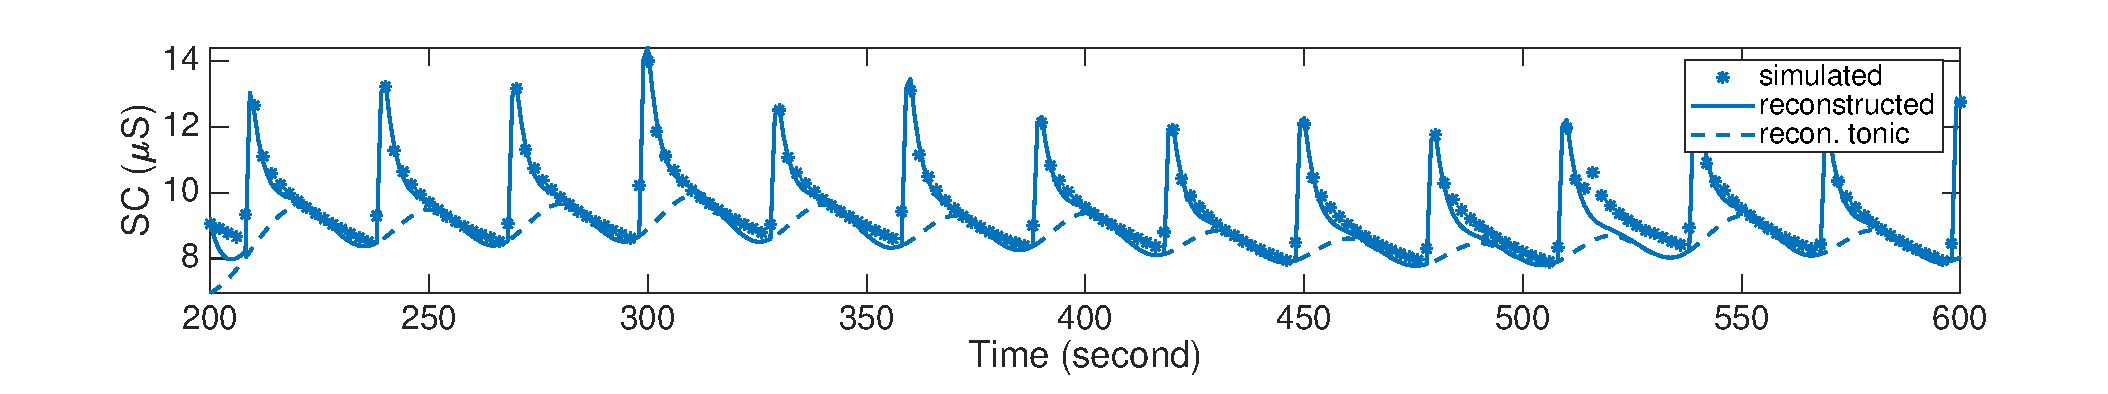
\includegraphics[width=0.9\textwidth]{middle_phalanx_3} \label{fig:middle_phalanx}}
  \subfigure[]{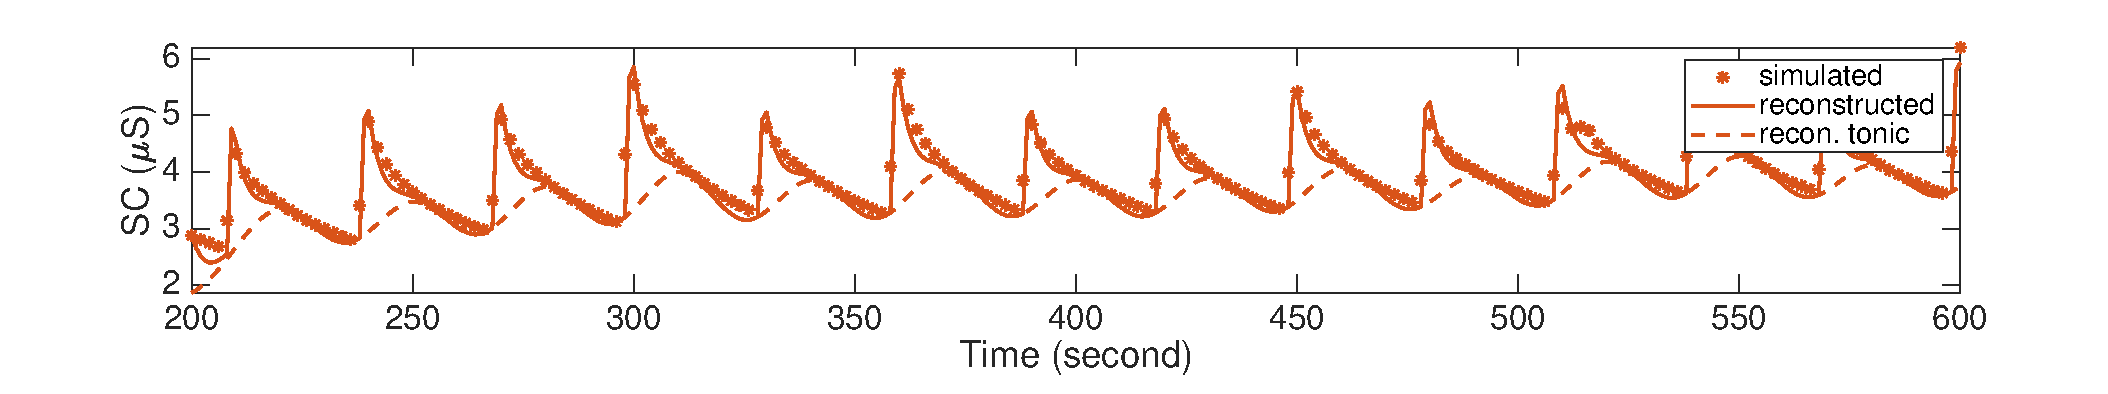
\includegraphics[width=0.9\textwidth]{medial_plantar_3} \label{fig:medial_plantar}}
  \subfigure[]{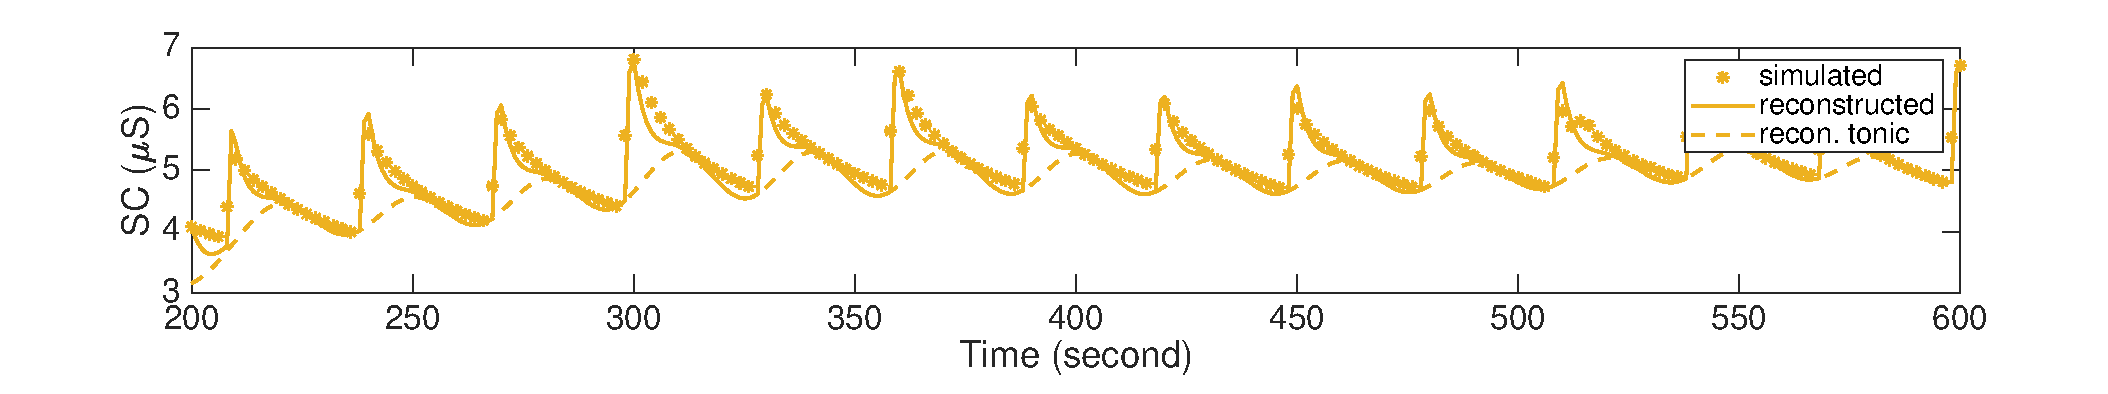
\includegraphics[width=0.9\textwidth]{thenar_3} \label{fig:thenar}}
  \subfigure[]{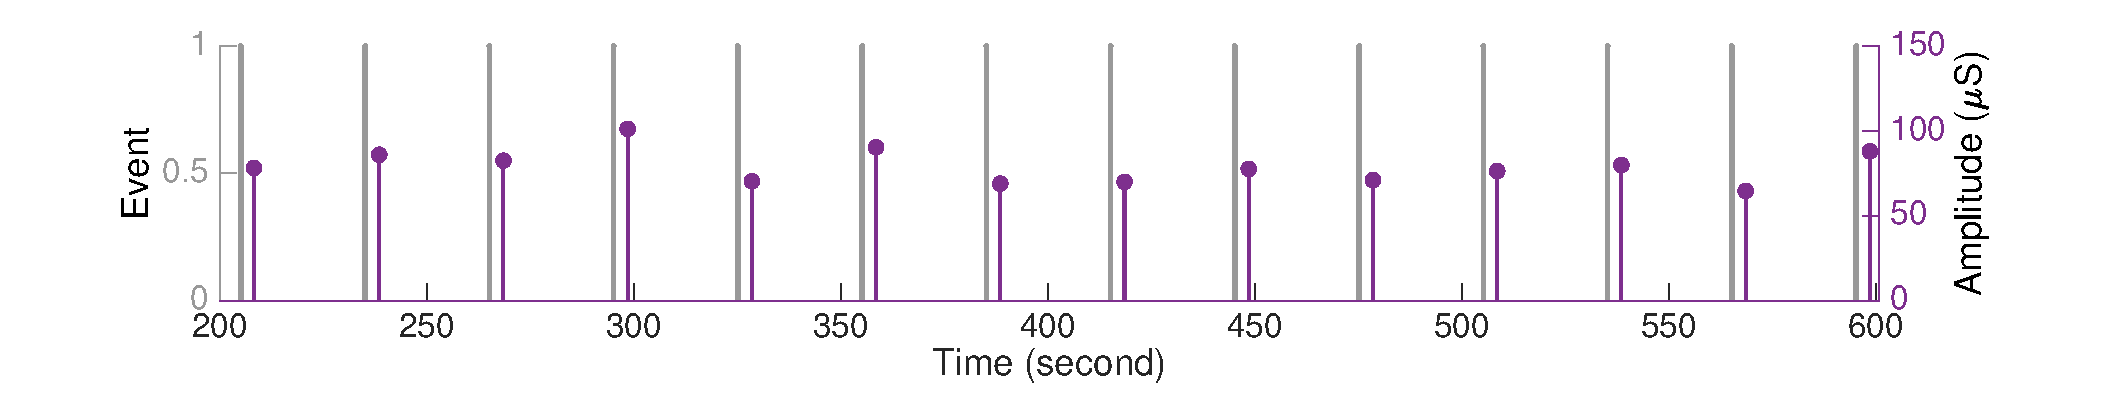
\includegraphics[width=0.9\textwidth]{stimuli_3} \label{fig:stimuli}}
  \DeclareGraphicsExtensions.
  \caption{The reconstructed signals for the data collected from the $11^{\mathrm{th}}$ participant. (a) The volar middle phalanx data. (b) The medial plantar surface data. (c) The thenar/hypothenar data. (d) The solved neural stimuli.} \label{fig:results}
\end{figure*}

Conventionally, it is difficult to decide the proper the regularization coefficients $\lambda,~\mu_n$. In our work, we take the optimization of the coefficients into the consideration. The optimization is based on Focal Underdetermined System Solver (FOCUSS+) algorithm~\cite{murray2005visual}, while the estimation of the tunable regularization coefficients is based on  generalized cross-validation (GCV) method~\cite{zdunek2008improved}. 

To solve the joint problem in \eqref{fml:the:optimization}, we need to divide the problem into two sub-problems and solve them alternatively. This technique is called concurrent coordinate descent method. The whole algorithm is discussed in \Cref{alg:deconvolution}. The algorithm has 2 phases. In the both phases, the tonic component and the phasic component are solved alternatively, the only difference is the regularization method. In the first phase, we make the initialization ratio fixed to simplify the algorithm. This phase is used for finding a good initialization. In the beginning of the initialization phase, we use conventional method to generate the tonic component bases, where the intervals between two basis are fixed.

In the second phase, the optimization could be divided into an outer loop and an inner loop. In the outer loop, we solve the modeling parameters $\boldsymbol{\theta}$. The deconvolution and with the tonic extraction is performed in the inner loop. Particularly, given the solution of $\{\mathbf{q}_n\}_{n=1}^{\chi}$, when solving the tonic component, for any $n$, we need to solve the following constrained quadratic problem,
\begin{subequations} \label{fml:the:second-tonic}
  \renewcommand{\theequation}
  {\theparentequation-\arabic{equation}}
  \begin{align}
    \argmin\limits_{\mathbf{q}_n,~\mu_n} & \lVert \mathbf{s}_n - \mathbf{S} \mathbf{q}_n \rVert^2_2 + \mu_n \lVert \mathbf{q}_n \rVert_2^2, \\
    \mathrm{s.t.}~& \mathbf{s}_n = \mathbf{y}_n - \mathcal{F}_{\boldsymbol{\theta}_n} \mathbf{z}_{0} - \mathcal{D}_{\boldsymbol{\theta}_n} \mathbf{u}, \label{fml:the:second-tonic-obj}\\
    & \forall~n,~\mathbf{q}_n \succcurlyeq \mathbf{0},~\mathbf{S}\mathbf{q}_n \preccurlyeq \mathbf{y}_n,
  \end{align}
\end{subequations}
%
where $\mathbf{S}\mathbf{q}_n$ is upper bounded by the signal $\mathbf{y}_n$. We do not set the upper bound by $\mathbf{s}_n$, because we do not require the positive residual for the solution of the phasic component.

When solving the phasic component, we make the tonic component fixed, and solve the following problem,
\begin{subequations} \label{fml:the:second-phasic}
  \renewcommand{\theequation}
  {\theparentequation-\arabic{equation}}
  \begin{align}
  \argmin\limits_{\boldsymbol{\theta},~\mathbf{u},~\lambda} & \frac{1}{\chi}  \left( \sum_{n=1}^{\chi} \lVert \mathbf{p}_n - \mathcal{F}_{\boldsymbol{\theta}_n} \mathbf{z}_{0} - \mathcal{D}_{\boldsymbol{\theta}_n} \rVert^2_2 \right) + \lambda \lVert \mathbf{u} \rVert_p^p, \\
  \mathrm{s.t.}~& \mathbf{p}_n = \mathbf{y}_n -  \mathbf{S} \mathbf{q}_n, \\
  & \boldsymbol{\Gamma} \boldsymbol{\theta} \preccurlyeq \mathbf{b},~ \mathbf{u} \succcurlyeq \mathbf{0}.
  \end{align}
\end{subequations}

\section{Results}

The dataset used in this work is called \texttt{PsPM-SCRV10}\cite{bach2014pspm}, where ``\texttt{PsPM}'' is the abbreviation of the organization ``Psycho-Physiological Modelling'', and ``\texttt{SCRV\_10}'' is the symbolic name of the dataset. This dataset is collected from an experiment. 26 volunteers (12 males and 14 females) are invited for participating the test. The researchers produce a series white noise bursts as auditory stimulations. In response, the participants are required to press a food pedal every time they hear the burst. The data is recorded by Cambridge Electronic Design (CED) spike software.

According to the type of the data, the dataset could be divided into two parts. The first part is called ``cogent''. It contains the record about the participants' reactions including which pedal they press and how long the pedal is pressed. This part is not related to our work. The second part is called ``spikes''. It is a collection of skin conductance response (SCR) measurements. We only use the following parts of the data:

\begin{enumerate}
  \item Marker denoting timings of the auditory stimulations;
  \item Skin conductance on the thenar/hypothenar of the non-dominant hand;
  \item Skin conductance on the volar middle phalanx of the dominant 2nd/3rd finger;
  \item Skin conductance on the medial plantar surface of the non-dominant foot;
\end{enumerate}

Since each volunteer could provides 3 SC data, we construct our model as a 3-channel one. The marker denoting the auditory stimulations are used as the ground truth for estimating our results.

To simplify the calculation, we downsample the data by setting $T_y=1\rm{s}$. The bin sizes of the stimuli $T_u$ are configured as 4s. For the tonic components, the knot size $\kappa$ is configured as $4s$, and the relatively delay time of the $T_{ds}$ is 25s. We take the results of the participant 11 as an example, where we extract the data from 200s to 600s. The results are shown in \Cref{fig:results}. In \Cref{fig:stimuli}, we draw the ground truth of the stimulation as gray bars and the solved neural stimuli as purple pins. The results show that the stimuli are always a little bit later than the stimulation. This phenomenon is reasonable, because there may be a latency caused by the physiological reactions. The solved parameters $\boldsymbol{\theta}$ are shown in \Cref{tab:theta}, where $\tau_r$ and $\tau_d$ are the rise and decay times, and $\alpha_2$ and $\alpha_3$ represent the relatively attenuation rates of the medial plantar surface data and the thenar/hypothenar data compared to the volar middle phalax data.

\begin{table}[h] 
  \centering
  \caption{The solve paramters $\boldsymbol{\theta}$ for the shown examples.} \label{tab:theta}
  \begin{tabular}{|c|c|c|c|c|}
    \hline
    Participant & $\tau_r$ & $\tau_d$ & $\alpha_{2}$ & $\alpha_{3}$ \\
    \hline
    11 & 0.2799s & 3.2583s & 0.4540 & 0.3844\\ \hline
    12 & 0.2799s & 3.2583s & 0.4540 & 0.3844\\
    \hline
  \end{tabular}
\end{table}

\section{Discussion}

The solutions in \Cref{fig:results} show a high fitness between the reconstructed signals and the raw data. By utilizing the multi-channel data, the influence of the noise is eliminated. For example, although there is an unfitness near 520s in \Cref{fig:middle_phalanx}, the other two channels could still achieve good fitness and suggest a correct impulse in the neural stimuli.

\begin{figure*}[!tb]
  \centering
  \subfigure[]{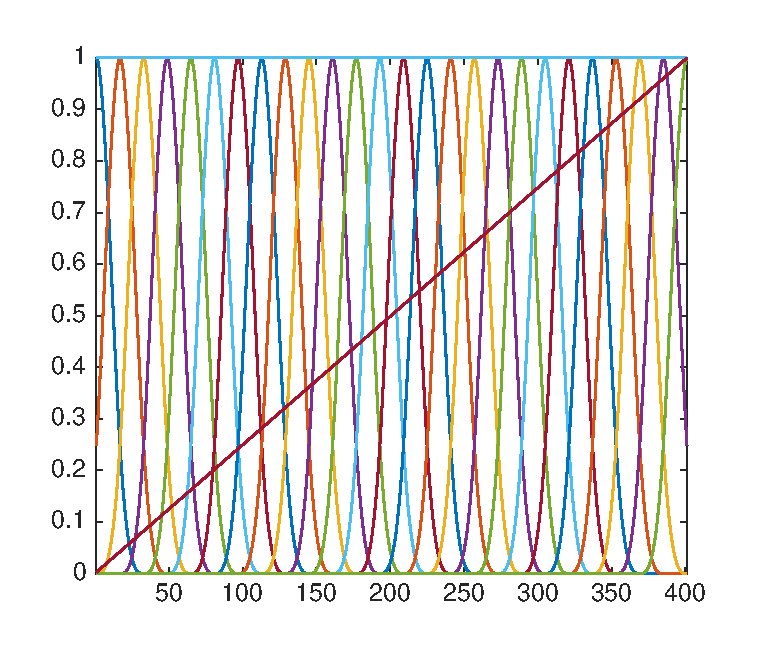
\includegraphics[width=0.7\columnwidth]{basis-c0} \label{fig:bases-c0}}
  \subfigure[]{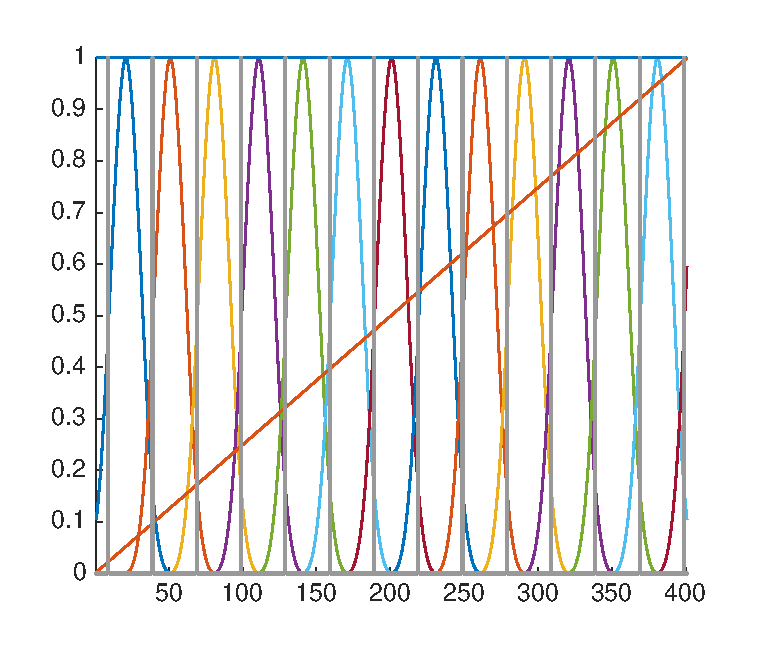
\includegraphics[width=0.7\columnwidth]{basis-c} \label{fig:bases-c}}
  \DeclareGraphicsExtensions.
  \caption{A comparison between the bases generated by different methods. We use the same knot size for both methods. (a) Conentional method, where the interval between bases is fixed. (b) Our method, where the positions of bases are relative to the solve neural stimuli.} \label{fig:bases}
\end{figure*}

\begin{figure*}[!tb]
  \centering
  \subfigure[]{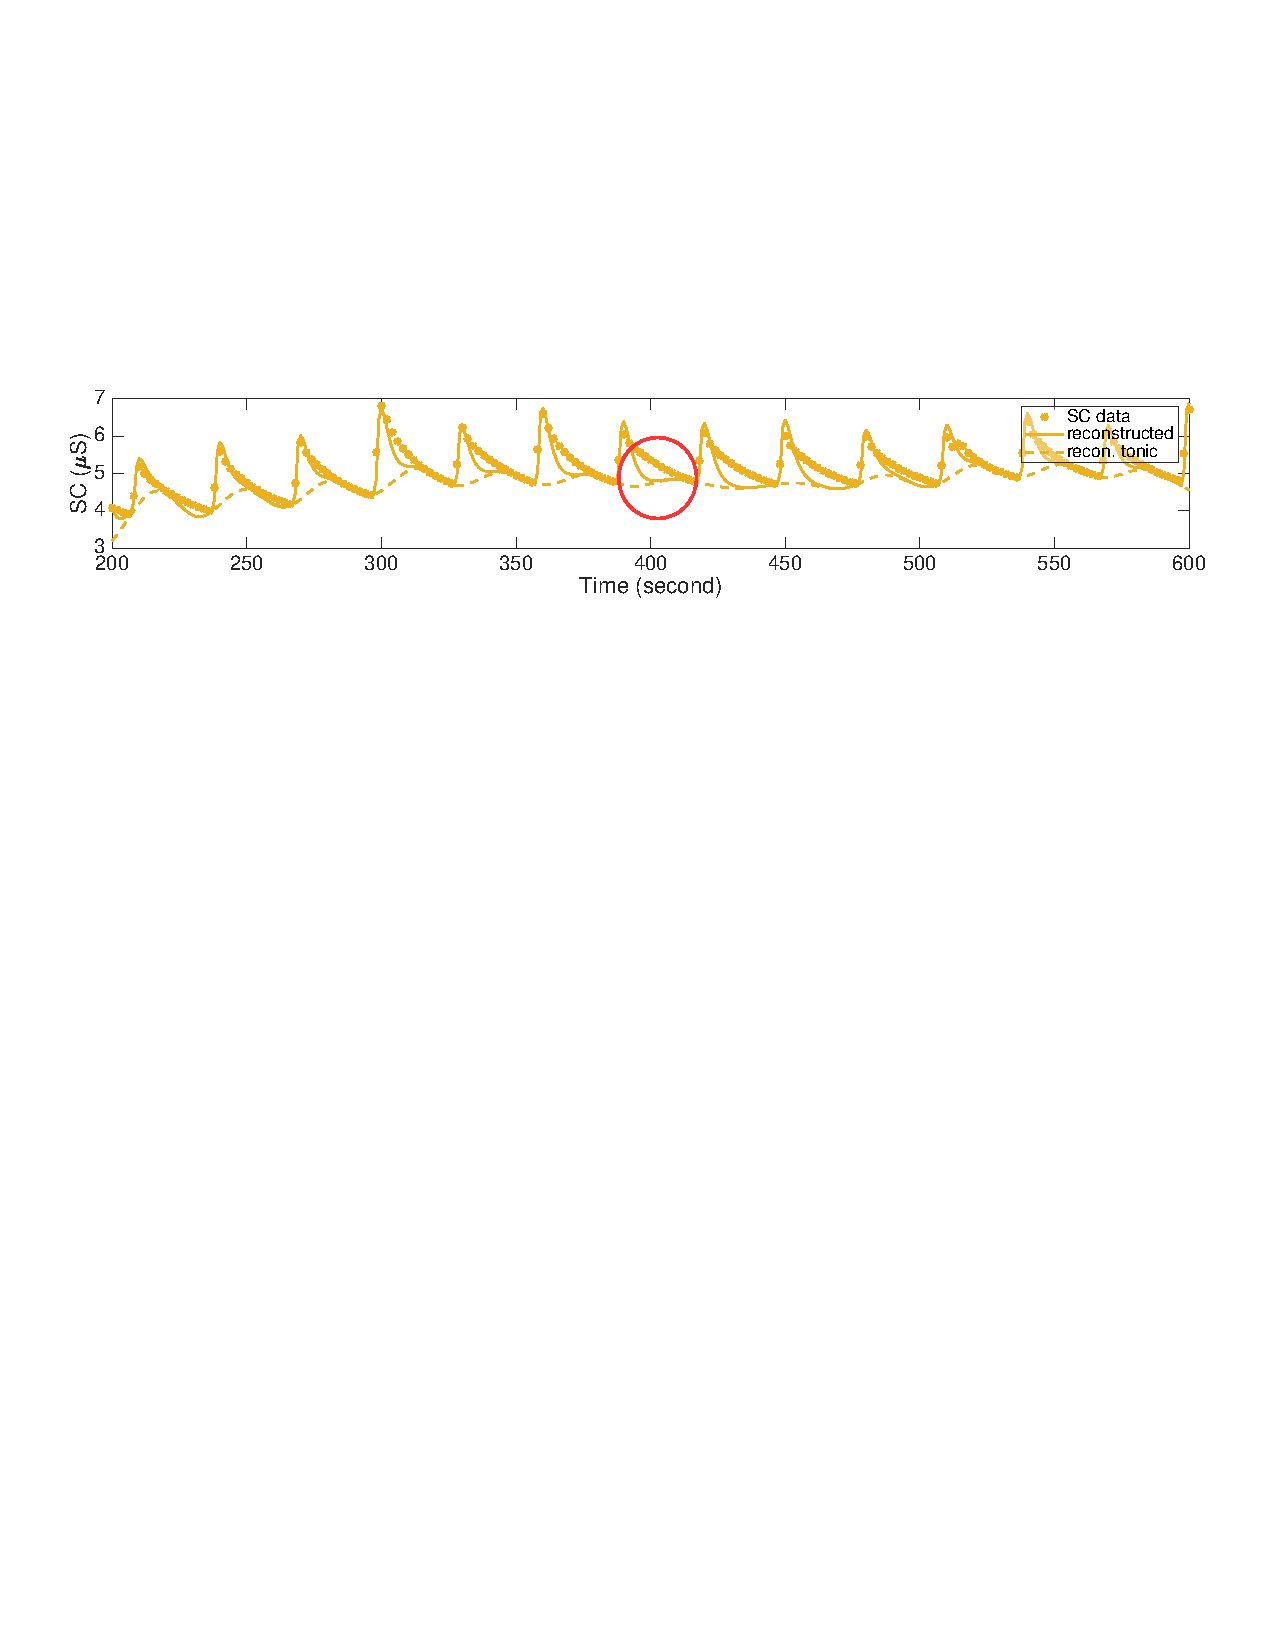
\includegraphics[width=0.9\textwidth]{thenar_bad}}
  \subfigure[]{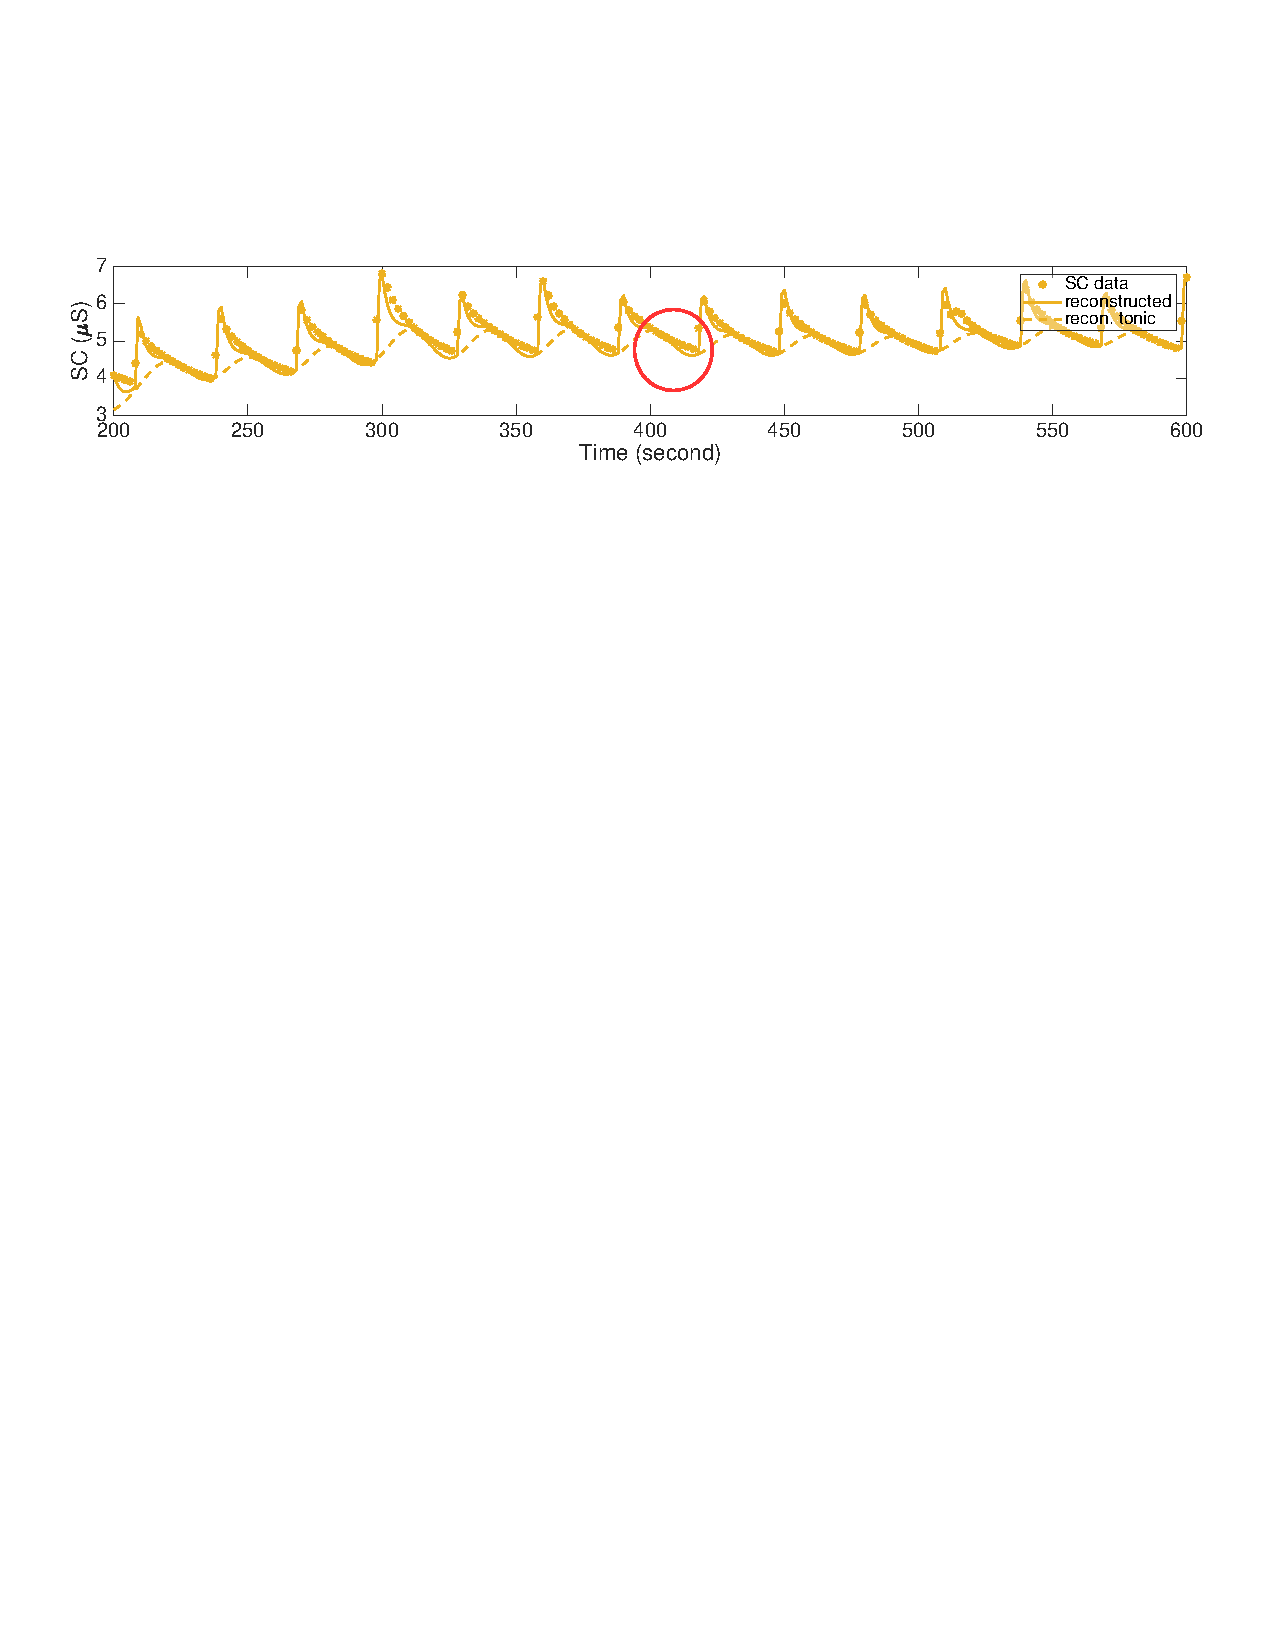
\includegraphics[width=0.9\textwidth]{thenar_3_good}}
  \DeclareGraphicsExtensions.
  \caption{Reconstructed signal for the thenar/hypothenar data of the participant 11 with different tonic extraction methods. (a) Conventional tonic extraction. (b) Our tonic extraction.} \label{fig:comptonic}
\end{figure*}

Experiments show that the fitness of the final solution is highly dependent of the quality of the solved tonic component. In previous works~\cite{greco2015cvxeda,amin2019tonic}, the B-spline bases are sampled by a fixed interval. In these methods, it is very tricky for determining how long the interval should be. If the interval is too small, there would be a deformation for the solved phasic component. If too large, the solved tonic component would be over-smoothed. According to \eqref{fml:the:ode}, since the neural stimuli are a series of sparse impulese, the phasic component is modeled by a series of peaks. According to \eqref{fml:tonic-conv}, the tonic component could be also viewed as a combination of B-spline peaks. Empirically, we find that when each peak of the tonic component appears a little bit later than the impulses of neural stimuli, the solution could reach the highest fitness. Inspired by this inspection, we propose the adaptive B-spline bases in \eqref{fml:tonic-basis-1}. In \Cref{fig:bases}, we compare the bases generated by the conventional method and our method when the shape of the bases are configured same. In \Cref{fig:bases-c}, we use gray lines to represent the location of the solved neural stimuli. We could find that the bases generated by our method is more sparse, and the position of each basis is related to the appearance of neural stimuli.

In \Cref{fig:comptonic}, we take the thenar/hypothenar data as an example. We perform two experiments with all the same configurations except for the tonic extraction methods. The results are produced by the fixed bases in \Cref{fig:bases-c0} and the adaptive bases in \Cref{fig:bases-c} respectively. With our method, the fitness is significantly improved in the region marked by red circles. In the conventional method, because the interval between bases is fixed, the marked tonic component peak is almost near the end of one phasic component peak. In comparison, our method ensures that the tonic component peak is nearly centered in the range of one phasic component peak.

Currently, we are using a fixed delay $T_{ds}$ for determining the relative position of the tonic bases, this may be not a best configuration. In the future work, we could make the delay for each basis learnable, and find the optimal relative delay by the algorithm. 

\section{Conclusion}

In this work, we try to combine the tonic component extraction and the multi-channel phasic component deconvolution together. The problem is formulated as a joint problem for solving both components. To solve this problem, we use the concurrent coordinate descent method. For the phasic component, we formulate the model by a state-space representation, and use FOCUSS+ to solve the neural stimuli with sparsity regularization. In comparison, the tonic component is modeled by the decomposition of B-spline functions, where the positions of the bases are adaptive. We use the interior point method to solve the constrained quadratic problem. The regularization ratio for both components are estimated by the GCV method. The final results show that the phasic component and tonic component are separated, and the neural stimuli is well-regularized by the sparsity.

\bibliographystyle{ieeetr}
\bibliography{ref}

\end{document}